% typedecide.tex -- IEEE conference format (IEEEtran, two-column).
% Build: `make` (uses tectonic). See ../README.md.
%
% PROVENANCE RULE: every number in this file is copied from bench/results/*.json,
% from a measurement recorded in README.md / paper/paper.md / packages/typedecide/docs/SPEED.md,
% or is exact arithmetic shown in the text. Numbers attributed to prior work
% are THEIR published numbers. Do not edit a number without editing its source.
\documentclass[conference]{IEEEtran}

% ---------------------------------------------------------------------------
% McNemar result, cyclic vs full-permutation averaging. Source: output of
%   node bench/compare.mjs \
%     results/authored144-Qwen3-0.6B-ONNX-q4f16-readout-cyclic-shots3.predictions.jsonl \
%     results/authored144-Qwen3-0.6B-ONNX-q4f16-readout-full-shots3.predictions.jsonl
% -> both right 69, only cyclic right 8, only full right 3, both wrong 64,
%    discordant pairs 11, exact McNemar p 0.2266  (= 2*(C(11,0)+..+C(11,3))/2^11 = 464/2048).
% If the prediction files are regenerated and these change, update the macros AND re-read
% Sec. VII-C: its prose assumes p > 0.05.
\newcommand{\mcnemarp}{0.23}
\newcommand{\mcnemardiscordant}{11}
\newcommand{\mcnemaronlycyclic}{8}
\newcommand{\mcnemaronlyfull}{3}
% Project repository, as given in packages/typedecide/README.md. Verify before submission.
\newcommand{\repourl}{\url{https://github.com/ardada2468/typedecide}}
% ---------------------------------------------------------------------------

\usepackage[T1]{fontenc}
\usepackage{cite}
\usepackage{amsmath,amssymb}
\usepackage{booktabs}
\usepackage{array}
\usepackage{xcolor}
\usepackage{url}
\usepackage{microtype}
\usepackage{tikz}
\usetikzlibrary{arrows.meta,positioning,calc,decorations.pathreplacing}
\usepackage{pgfplots}
\pgfplotsset{compat=1.17}

\newcommand{\code}[1]{\texttt{\small #1}}
\newcommand{\measured}{\textsc{measured}}
\newcommand{\derived}{\textsc{derived}}
\newcommand{\projected}{\textsc{projected}}
\hyphenation{to-ken-izer to-ken-izers read-out}

\begin{document}

\title{Typed Decisions in the Browser: What Limits Logit Readout on Sub-1B Language Models}

\author{\IEEEauthorblockN{Arnav Dadarya}
\IEEEauthorblockA{\textit{[AFFILIATION PLACEHOLDER --- department, institution]}\\
\textit{[PLACEHOLDER --- city, country]}\\
arnavdadarya@gmail.com}}

\maketitle

\begin{abstract}
Many decisions that software delegates to a language model are small and closed: route a ticket, judge whether a claim is supported. Instead of generating text and parsing it, a \emph{typed logit readout} lists the options as lettered slots and takes a softmax over the answer-letter logits at one position. We implement this client-side (transformers.js on ONNX Runtime, Qwen3-0.6B, 4-bit weights) and measure what limits it: (i) batched branch evaluation, which makes the server-side form efficient, is rejected by ONNX Runtime's fused attention kernel, so criteria are scored serially; (ii) shared-prefix KV reuse is bit-exact in fp32; (iii) on the public 144-row \emph{authored144} fixture, generation and readout score identically (0.419 mean family balanced accuracy): the readout buys closed support, determinism and a per-option distribution, not accuracy; (iv) averaging over option orderings raises the score to 0.483 (cyclic) or 0.442 (full permutation), which an exact McNemar test cannot distinguish at $n=144$ ($p=\mcnemarp$), while 87 of 144 rows still change their answer under rotation. Debiasing does not close the gap to the 0.813 published for a 4B model. No fine-tuned, trimmed or pruned model was evaluated.
\end{abstract}

\begin{IEEEkeywords}
language models, multiple-choice position bias, logit readout, contextual calibration, permutation averaging, KV-cache reuse, on-device inference, WebGPU, negative result
\end{IEEEkeywords}

% ===========================================================================
\section{Introduction}
A large share of the decisions that applications ask a language model to make are small and closed: \emph{which queue should handle this ticket, is this claim supported by the evidence, does this request need approval}. The conventional implementation asks a chat model to emit JSON and parses it back into control flow. That spends decode steps on tokens the caller discards and, without constrained decoding~\cite{willard2023guided}, gives no structural guarantee that the emitted value is one of the permitted ones.

An alternative is to present the options as lettered slots and read the probability distribution over the token ids of those letters at a single position~\cite{robinson2023mcqa}. Nothing is sampled, so nothing can be malformed, and the distribution ranges only over the options supplied. Existing open implementations of this pattern were developed and benchmarked server-side on a GPU~\cite{openjev,archerhume}.

Our question is what the technique is worth when it runs \emph{on the user's device}, where there is no server, no per-token fee, and the text never leaves the tab---and, separately, what limits its accuracy at the model sizes that fit there. This is a short empirical paper. It does not propose a new model or a new debiasing method; permutation averaging and contextual calibration are prior work~\cite{zheng2024selectors,zhao2021calibrate}. Its value is in the measurements, including the ones that came out against us.

\textbf{Contributions.}
\begin{enumerate}
\item A browser-native implementation of typed logit readout in which answer-slot token ids are \emph{discovered} from the tokenizer at run time rather than hardcoded, and in which shared-prefix KV reuse is verified bit-exact in fp32 (Sec.~\ref{sec:design}).
\item A negative engineering result: batched branch evaluation against a shared past KV cache is rejected by ONNX Runtime's \code{GroupQueryAttention} kernel, so the ``flat in the number of criteria'' scaling of the server-side form does not transfer to this browser stack (Sec.~\ref{sec:negative}).
\item A controlled ablation on a public fixture showing that (a) generation and readout score \emph{identically}, (b) option-order sensitivity is large---87 of 144 decisions change under rotation---and invisible to plain accuracy, and (c) cyclic permutation averaging recovers 6.4 points, which is not statistically separable from full permutation averaging and does not close the gap to larger models (Sec.~\ref{sec:results}).
\item A cost argument, specific to prefix-reused readout, for why $K$-ordering debiasing costs $K$ short suffixes rather than $K$ full prompts, with a measured linear suffix-cost model (Sec.~\ref{sec:debias}, \ref{sec:cost}).
\item \code{typedecide}, an open library for bringing one's own decision data, fine-tuning on the answer token only, evaluating with order-robust metrics and exporting to the browser (Sec.~\ref{sec:library}). We state up front that \emph{no fine-tuned model has been trained or evaluated with it for this paper}.
\end{enumerate}

% ===========================================================================
\section{Background and Related Work}
\subsection{Typed logit readout}
Given a state $s$, a question $q$ and options $o_1,\dots,o_n$, the prompt lists the options as \code{A.}, \code{B.}, \dots\ and ends at \code{Answer:}. Let $t_i$ be the token id the tokenizer produces for letter $i$ \emph{at that exact prompt boundary}, and $\ell\in\mathbb{R}^{|V|}$ the logits at the final position. The decision is the restricted softmax
\begin{equation}
P(o_i \mid s,q) \;=\; \frac{\exp \ell_{t_i}}{\sum_{j=1}^{n}\exp \ell_{t_j}} .
\label{eq:readout}
\end{equation}
Two properties follow directly: the support is exactly the supplied options, and the result is deterministic. Robinson \emph{et al.}~\cite{robinson2023mcqa} studied this ``multiple-choice prompting'' against cloze-style scoring of option text; scoring the text directly suffers from surface-form competition~\cite{holtzman2021surface} and from multi-token options that share prefixes. We therefore score letters, never option text. Constrained (guided) decoding~\cite{willard2023guided} is the generation-side route to the same closed-support guarantee; we did not benchmark it.

\subsection{Prior implementations}\label{sec:prior}
The letter-slot readout, the practice of verifying the shared prefix at token level, and the public fixture and metric used in Sec.~\ref{sec:setup} come from prior open-source work~\cite{openjev}, which also ships a browser demo built on wllama~\cite{wllama}. It runs BF16 server-side and reports that shared-prefix scoring is not bit-exact in that format~\cite{openjev}. We did not run the closed hosted service that popularised the interface~\cite{archerhume} and make no claim about it.

\subsection{Position bias and calibration in multiple choice}
That language models answering multiple-choice questions are sensitive to the order and labelling of options is well documented. Zhao \emph{et al.}~\cite{zhao2021calibrate} showed that few-shot predictions carry systematic biases that can be estimated with a content-free input and divided out (\emph{contextual calibration}). Pezeshkpour and Hruschka~\cite{pezeshkpour2024order} measured large accuracy swings from reordering options alone. Zheng \emph{et al.}~\cite{zheng2024selectors} attribute much of the effect to a prior over option \emph{ID tokens}, and use cyclic and full permutation averaging as (costly) debiasing baselines for their cheaper estimator. We adopt cyclic and full permutation averaging and contextual calibration unchanged; what is specific to our setting is their cost structure under prefix reuse (Sec.~\ref{sec:debias}) and their behaviour on a sub-1B model.

\subsection{Prefix sharing}
Reusing attention key/value state for a shared prompt prefix is standard in LLM serving, e.g.\ block-level sharing in PagedAttention~\cite{kwon2023paged}. The models we use employ grouped-query attention~\cite{ainslie2023gqa}, which is relevant only because the fused kernel implementing it is where the negative result of Sec.~\ref{sec:negative} arises.

% ===========================================================================
\section{System Design}\label{sec:design}
The system is a static web page: no backend, no build step, and no network traffic after the weights are cached. Inference is transformers.js~\cite{transformersjs} (v4.3.0) over ONNX Runtime~\cite{onnxruntime}, on WebGPU when available and WebAssembly otherwise. Fig.~\ref{fig:arch} contrasts it with the generation baseline that the same page also runs.

\begin{figure}[t]
\centering
% Fig. 1 -- system architecture. Conceptual diagram; no measured data.
% Mirrors web/engine.js: Engine.prefill() -> Engine.score() -> readSlots(), and
% Engine.generate() -> firstJsonObject() -> auditJson() for the generation lane.
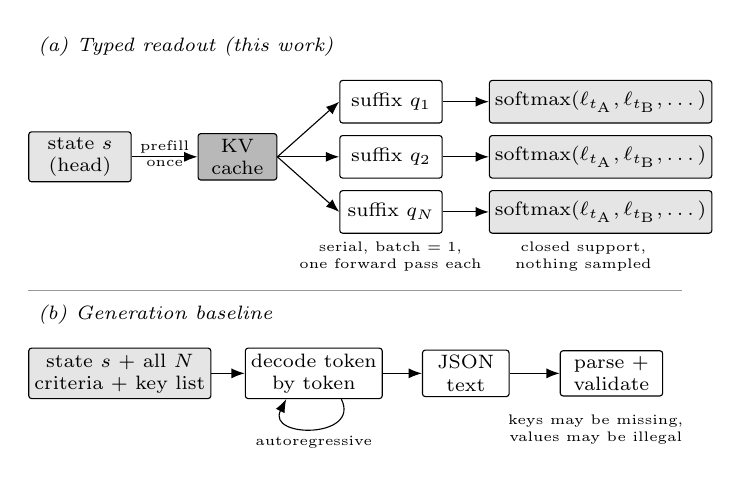
\begin{tikzpicture}[
    font=\scriptsize, >=Latex,
    box/.style={draw, rounded corners=1pt, align=center, inner sep=2pt, minimum height=5.4mm},
    lite/.style={box, fill=black!10},
    dark/.style={box, fill=black!28},
    lab/.style={font=\scriptsize\itshape, anchor=west}]
  % ---------------- (a) readout path
  \node[lab] at (0,0.95) {(a) Typed readout (this work)};
  \node[lite, minimum width=13mm, anchor=west] (state) at (0,-0.45) {state $s$\\(head)};
  \node[dark, minimum width=10mm, anchor=west] (kv) at (2.15,-0.45) {KV\\cache};
  \draw[->] (state) -- node[above, font=\tiny, inner sep=1pt]{prefill} node[below, font=\tiny, inner sep=1pt]{once} (kv);
  \foreach \i/\y/\q in {1/0.25/1, 2/-0.45/2, 3/-1.15/N} {
    \node[box, minimum width=13mm, anchor=west] (c\i) at (3.95,\y) {suffix $q_{\q}$};
    \node[lite, minimum width=24mm, anchor=west] (s\i) at (5.85,\y) {softmax$(\ell_{t_{\mathrm A}},\ell_{t_{\mathrm B}},\dots)$};
    \draw[->] (kv.east) -- (c\i.west);
    \draw[->] (c\i) -- (s\i);
  }
  \node[font=\tiny, align=center] at (4.6,-1.72) {serial, batch $=1$,\\one forward pass each};
  \node[font=\tiny, align=center] at (7.05,-1.72) {closed support,\\nothing sampled};
  % ---------------- (b) generation path
  \draw[black!40] (0,-2.15) -- (8.3,-2.15);
  \node[lab] at (0,-2.45) {(b) Generation baseline};
  \node[lite, minimum width=21mm, anchor=west] (full) at (0,-3.2) {state $s$ + all $N$\\criteria + key list};
  \node[box, minimum width=16mm, anchor=west] (dec) at (2.75,-3.2) {decode token\\by token};
  \node[box, minimum width=11mm, anchor=west] (json) at (5.0,-3.2) {JSON\\text};
  \node[box, minimum width=13mm, anchor=west] (parse) at (6.75,-3.2) {parse +\\validate};
  \draw[->] (full) -- (dec); \draw[->] (dec) -- (json); \draw[->] (json) -- (parse);
  \draw[->] ($(dec.south)+(0.35,0)$) .. controls +(0.25,-0.5) and +(-0.25,-0.5) .. ($(dec.south)+(-0.35,0)$);
  \node[font=\tiny] at ($(dec.south)+(0,-0.55)$) {autoregressive};
  \node[font=\tiny, align=center] at ($(parse.south)+(-0.2,-0.42)$) {keys may be missing,\\values may be illegal};
\end{tikzpicture}

\caption{(a) The state is prefilled once; each criterion is a short suffix scored against the same KV cache and read with a restricted softmax, Eq.~\eqref{eq:readout}. Branches are scored serially (Sec.~\ref{sec:negative}). (b) The generation baseline emits one JSON object answering all criteria, which must then be parsed and validated.}
\label{fig:arch}
\end{figure}

\subsection{Prompt layout}
The prompt is split into a \emph{head} shared by every criterion asked about one state and a per-criterion \emph{tail} (Fig.~\ref{fig:prompt}). The head holds a fixed instruction and the evidence; the tail holds the question, the lettered options and the literal \code{Answer:}. The same prompt-building code is imported by the browser engine and by the benchmark harness, and the Python library mirrors it byte for byte with a CI parity check, because a model fine-tuned against a prompt that deployment never sends degrades silently.

\begin{figure}[t]
\centering
% Fig. 2 -- prompt anatomy. Text follows web/prompt.js (INSTRUCTION, headText, tailText).
% The example state/criterion are from bench/shared_check.mjs (abbreviated).
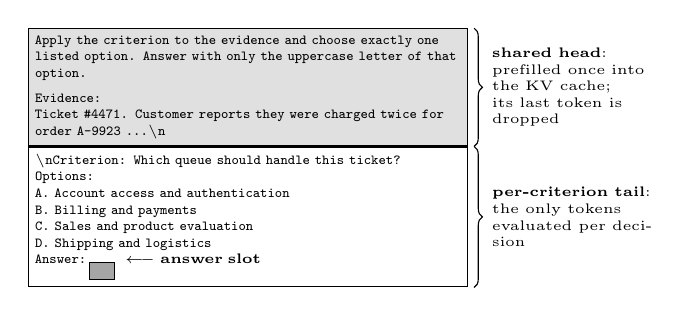
\begin{tikzpicture}[font=\scriptsize]
  \def\W{54mm}
  \node[draw, fill=black!12, text width=\W, inner sep=2.5pt, align=left, anchor=north west, font=\ttfamily\tiny] (head) at (0,0) {%
    Apply the criterion to the evidence and choose exactly one listed option. Answer with only the uppercase letter of that option.\\[3pt]
    Evidence:\\
    Ticket \#4471. Customer reports they were charged twice for order A-9923 \dots\textbackslash n};
  \node[draw, text width=\W, inner sep=2.5pt, align=left, anchor=north west, font=\ttfamily\tiny] (tail) at (head.south west) {%
    \textbackslash nCriterion: Which queue should handle this ticket?\\
    Options:\\
    A. Account access and authentication\\
    B. Billing and payments\\
    C. Sales and product evaluation\\
    D. Shipping and logistics\\
    Answer:\,\tikz[baseline=-0.4ex]{\node[draw, fill=black!35, minimum width=3.2mm, minimum height=2.2mm, inner sep=0pt]{};}%
    \ \ {\normalfont\tiny$\longleftarrow$ \textbf{answer slot}}};
  \draw[decorate, decoration={brace, amplitude=3pt}] ($(head.north east)+(0.8mm,0)$) -- ($(head.south east)+(0.8mm,0)$)
    node[midway, right=3pt, align=left, text width=21mm, font=\tiny] {\textbf{shared head}:\\ prefilled once into the KV cache; its last token is dropped};
  \draw[decorate, decoration={brace, amplitude=3pt}] ($(tail.north east)+(0.8mm,0)$) -- ($(tail.south east)+(0.8mm,0)$)
    node[midway, right=3pt, align=left, text width=21mm, font=\tiny] {\textbf{per-criterion tail}:\\ the only tokens evaluated per decision};
\end{tikzpicture}

\caption{Prompt anatomy. Grey: shared head. White: per-criterion tail. The readout uses only the logits at the final position.}
\label{fig:prompt}
\end{figure}

\subsection{Answer slots are discovered, not assumed}
Prior browser implementations ship the answer-letter token ids as configuration as a per-model base id plus the letter index~\cite{openjev}. This is fragile. The ids are not contiguous in any vocabulary we checked: for Gemma~3~\cite{gemma3}, the letters \code{A,B,C,D} resolved to ids $562, 603, 565, 622$, so a \code{labelBase + index} shortcut (which would give $562,563,564,565$) is silently wrong for every letter after \code{A}. Whether the natural continuation after \code{Answer:} is \code{" A"} or \code{"A"} also depends on the tokenizer and the preceding character.

For each prompt we therefore probe both separators against the real tokenizer and keep the first for which appending each letter (i) adds exactly one token, (ii) leaves the tokenization of the prompt itself unchanged, and (iii) yields distinct ids; if neither separator satisfies all three, scoring aborts rather than guessing. The cost is a handful of \code{encode} calls per criterion. The engine also reports the \emph{allowed mass}, the share of the full-vocabulary softmax that falls on the answer letters, as a diagnostic of whether the model has adopted the output format.

\subsection{Shared-prefix KV reuse and the drop-last-token rule}\label{sec:prefix}
The head is prefilled once and its \code{present.*} tensors are passed back as \code{past\_key\_values} for every criterion, never mutated. Correctness requires the cached ids to be an exact \emph{token-level} prefix of every full prompt, which string concatenation does not guarantee: the first character of the tail can merge with the last token of the head. Following prior practice~\cite{openjev}, we drop the final head token before prefilling, and at scoring time we tokenize the \emph{full} prompt, verify that the cached ids are a prefix of it (aborting otherwise), and feed the remainder as the suffix.

\subsection{Serial branch scoring}
Each criterion is one forward pass with batch size one: suffix ids in, one position of logits read. Criteria are independent, so results stream to the caller as they complete; the first decision is available after one prefill and one suffix pass.

% ===========================================================================
\section{A Negative Result: No Batched Branching}\label{sec:negative}
The server-side form replicates the prefix KV across a batch and evaluates every criterion in one padded forward pass, which makes total time roughly flat in the number of criteria~\cite{openjev}. We attempted the same through ONNX Runtime and it is refused outright:

\begin{quote}\small\ttfamily\raggedright
GroupQueryAttention: batch\_size must be 1 when sequence\_length > 1 and past context is given.
\end{quote}

The fused attention kernel admits a batch wider than one only when \emph{no} past KV is supplied---the one case where batching buys nothing here, because the shared evidence would be re-prefilled for every criterion. wllama, the other common browser runtime, exposes no batched branch evaluation either, for unrelated reasons. With this stack, therefore, criteria are scored serially and total time is linear in the number of criteria. What the shared prefill buys is a \emph{shorter prompt per decision}, not a single forward pass. Claims of ``one batched pass, $N$ decisions'' belong to a server implementation and do not transfer. We record the error as observed during development; we have not audited other ONNX Runtime versions or non-fused attention exports, either of which might lift the restriction.

% ===========================================================================
\section{Debiasing Methods}\label{sec:debias}
Let $\Pi$ be a set of orderings of the $n$ options and $P_\pi(o)$ the probability that Eq.~\eqref{eq:readout} assigns to option \emph{identity} $o$ when the prompt lists the options in order $\pi$.

\subsection{Permutation averaging}
We average per identity and take the argmax:
\begin{equation}
\bar P(o) = \frac{1}{|\Pi|}\sum_{\pi\in\Pi} P_\pi(o), \qquad \hat o = \arg\max_{o}\bar P(o).
\label{eq:avg}
\end{equation}
\emph{Cyclic} averaging uses the $n$ rotations $\pi_k(i) = (i+k) \bmod n$, $k=0,\dots,n-1$; \emph{full} averaging uses all $n!$ orderings. Both are balanced in the sense of Fig.~\ref{fig:cyclic}: each option occupies each slot equally often (once under cyclic, $(n-1)!$ times under full). If the slot prior is additive in probability, $P_\pi(o) = f(o) + g(\mathrm{slot}_\pi(o))$, then
\begin{equation}
\bar P(o) = f(o) + \frac{1}{n}\sum_{j=1}^{n} g(j),
\label{eq:cancel}
\end{equation}
and the second term is identical for every option, so it cannot change the argmax. We note a caveat: if the prior is instead additive in \emph{logit} space, arithmetic averaging of probabilities cancels it only to first order (the geometric mean would cancel it exactly). Our implementation averages probabilities as in Eq.~\eqref{eq:avg}; we did not evaluate log-space averaging.

\begin{figure}[t]
\centering
% Fig. 5 -- cyclic rotation as a Latin square. Conceptual; mirrors cyclic(n) in
% bench/authored144.mjs: order_k[i] = (i + k) mod n.
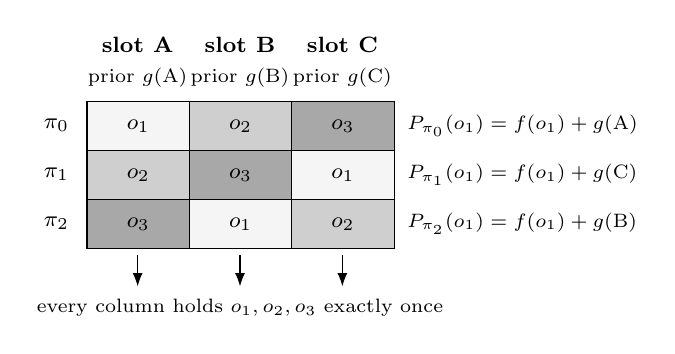
\begin{tikzpicture}[font=\footnotesize,
    cell/.style={draw, minimum width=13mm, minimum height=6.2mm, inner sep=0pt, anchor=north west}]
  \foreach \j/\L in {0/A,1/B,2/C} {
    \node[font=\footnotesize\bfseries] at (\j*1.3+0.65, 0.72) {slot \L};
    \node[font=\scriptsize] at (\j*1.3+0.65, 0.3) {prior $g(\mathrm{\L})$};
  }
  \foreach \k/\a/\b/\c in {0/1/2/3, 1/2/3/1, 2/3/1/2} {
    \node[anchor=east] at (-0.1, -\k*0.62-0.31) {$\pi_{\k}$};
    \foreach \j/\o in {0/\a,1/\b,2/\c} {
      \pgfmathtruncatemacro{\g}{(\o-1)*15+4}
      \node[cell, fill=black!\g] at (\j*1.3, -\k*0.62) {$o_{\o}$};
    }
  }
  \foreach \j in {0,1,2} {
    \draw[->, >=Latex] (\j*1.3+0.65,-1.95) -- (\j*1.3+0.65,-2.35);
  }
  \node[font=\scriptsize, align=center] at (1.95,-2.62) {every column holds $o_1,o_2,o_3$ exactly once};
  \node[anchor=west, font=\scriptsize, align=left] at (3.95,-0.31) {$P_{\pi_0}(o_1)=f(o_1)+g(\mathrm A)$};
  \node[anchor=west, font=\scriptsize, align=left] at (3.95,-0.93) {$P_{\pi_1}(o_1)=f(o_1)+g(\mathrm C)$};
  \node[anchor=west, font=\scriptsize, align=left] at (3.95,-1.55) {$P_{\pi_2}(o_1)=f(o_1)+g(\mathrm B)$};
\end{tikzpicture}

\caption{Cyclic rotation for $n=3$ is a Latin square over (ordering, slot): each option visits each slot once. Under an additive slot prior $g$, every option therefore collects the same total $g(\mathrm A)+g(\mathrm B)+g(\mathrm C)$ (shown at right for $o_1$), which shifts all averaged scores equally and cannot change the argmax, Eq.~\eqref{eq:cancel}.}
\label{fig:cyclic}
\end{figure}

\subsection{Contextual calibration}
Following Zhao \emph{et al.}~\cite{zhao2021calibrate}, we estimate the prior of an ordering directly by scoring the same question and ordering with the evidence replaced by a content-free state $s_\varnothing$ (the string \code{N/A}), and divide it out:
\begin{equation}
\tilde P_\pi(o) = \frac{P_\pi(o\mid s)\,/\,\max\!\big(P_\pi(o\mid s_\varnothing),\epsilon\big)}{\sum_{o'} P_\pi(o'\mid s)\,/\,\max\!\big(P_\pi(o'\mid s_\varnothing),\epsilon\big)},
\label{eq:calib}
\end{equation}
with $\epsilon=10^{-9}$. The null distribution is cached per (question, ordering). \emph{As implemented in our harness, the calibrated mode applies Eq.~\eqref{eq:calib} to each of the $n$ cyclic orderings and then averages them with Eq.~\eqref{eq:avg}}; the row labelled ``calibration'' in Sec.~\ref{sec:results} is therefore calibration \emph{combined with} cyclic averaging, not calibration of a single ordering. We did not run single-ordering calibration.

\subsection{Order instability}
Whenever more than one ordering is scored, we also record whether the per-ordering argmax \emph{identity} is the same under all of them. A row is \emph{order-unstable} if it is not. This is a property of the model's individual answers; averaging does not change it.

\subsection{Cost: $K$ suffixes, not $K$ prompts}\label{sec:costarg}
Every ordering changes only the option block, which lives in the tail. With a head of $L$ tokens prefilled once, tails of $m$ tokens, $N$ criteria and $K$ orderings, the readout costs
\begin{equation}
T_{\text{reuse}} = T_{\text{pre}}(L) + N K\,T_{\text{suf}}(m),
\label{eq:cost}
\end{equation}
against $N K\,T_{\text{pre}}(L+m)$ without reuse. A generation-based system has no equivalent: re-asking under $K$ orderings means $K$ complete requests, each with its own decode. Sec.~\ref{sec:cost} measures $T_{\text{suf}}$. This is a structural argument supported by that measurement; as stated in Sec.~\ref{sec:setup}, the accuracy harness itself does \emph{not} use prefix reuse, so its wall-clock times are not a demonstration of Eq.~\eqref{eq:cost}.

% ===========================================================================
\section{Experimental Setup}\label{sec:setup}
\textbf{Fixture.} All accuracy numbers are on the public \emph{authored144} fixture~\cite{openjev}: 144 authored decisions in three families---evidence interpretation, rule application, candidate selection---of 48 rows each, with three options per row, so chance is $1/3$. The fixture varies the position of the gold option across rows (gold is in slot A/B/C for 55/44/45 rows), so a fixed-letter answerer is penalised. We use a public fixture deliberately: it has published numbers for several models, which places our results on a scale we did not build. We do not redistribute it. Its provenance fields mark every row as synthetic, authored, and model-reviewed rather than human-adjudicated.

\textbf{Metric.} Following the fixture's metric contract~\cite{openjev}, we report \emph{mean family balanced accuracy}. With families $F$, gold classes $C_f$ in family $f$, and $N_{f,c}$ rows of gold class $c$ of which $\mathrm{TP}_{f,c}$ are predicted correctly,
\begin{equation}
\mathrm{MFBA} = \frac{1}{|F|}\sum_{f\in F}\;\frac{1}{|C_f|}\sum_{c\in C_f}\frac{\mathrm{TP}_{f,c}}{N_{f,c}} .
\label{eq:mfba}
\end{equation}
Balanced accuracy~\cite{brodersen2010balanced} is used because classes are uneven (e.g.\ 21/12/15 in evidence interpretation) and a majority-class answerer should not score well. We also report plain accuracy and the count of order-unstable rows.

\textbf{Model.} We use Qwen3-0.6B~\cite{qwen3} in the community ONNX export \code{onnx-community/Qwen3-0.6B-ONNX} at \code{q4f16} (4-bit block-quantised weights, fp16 compute), the same artefact the web page loads on WebGPU. It is used as a completion model with no chat template. The accuracy cost of this quantisation relative to fp16/fp32 was not measured.

\textbf{Prompting.} Zero or three demonstrations precede the prompt. The demonstrations are project-authored, not rows of the fixture, and their gold letters are C, B and B (no demonstration has gold A); the first demonstration uses the same three option descriptions as the fixture's evidence-interpretation family. The generation baseline receives the identical prompt, decodes greedily for at most six tokens, and the first capital letter in the output is parsed as the answer.

\textbf{Harness and hardware.} Accuracy runs are made by the script \code{bench/authored144.mjs} under Node, with transformers.js 4.3.0 on \code{onnxruntime-node} (CPU), on a single MacBook laptop; the exact model of the machine was not recorded. For simplicity the harness scores every ordering as a \emph{full prompt from scratch}, without prefix reuse; Sec.~\ref{sec:exact} establishes that this yields the same probabilities. The cyclic and full-permutation configurations were run twice, with identical accuracy (Sec.~\ref{sec:unresolved}); the others once. Wall-clock times are from single runs on an otherwise uncontrolled laptop. Browser latencies (Sec.~\ref{sec:browser}) are from the demo page on WebGPU, also on a MacBook, and are not comparable to the CPU figures.

\textbf{Comparison numbers.} The fixture's authors publish, on the same fixture and metric, 0.440 for Qwen3-0.6B, 0.686 for MiniCPM5-2B and 0.813 for Qwen3.5-4B~\cite{openjev}. These are \emph{their} measurements, on their hardware, scored natively in BF16 with their prompt (their table lists Q8\_0 and Q4\_K\_M GGUF files as the corresponding browser artefacts). We did not reproduce them, and neither numeric format nor prompt is controlled across the comparison.

\textbf{Significance.} For the one ranking that is contested (Sec.~\ref{sec:unresolved}) we use an exact two-sided McNemar test~\cite{mcnemar1947,dietterich1998tests} on per-row correctness: with $b$ and $c$ the rows that only one of the two methods gets right, $p=\min\!\big(1,\,2\sum_{k=0}^{\min(b,c)}\binom{b+c}{k}2^{-(b+c)}\big)$.

% ===========================================================================
\section{Results}\label{sec:results}

\subsection{An eight-item probe: position priors at small scale}
The measurement that motivated the rest. Eight unambiguous decisions (three with three options, five with two) were scored under every rotation of their option list, 19 prompts in all, so the expected accuracy of a uniform guesser is $(3\cdot\tfrac13+5\cdot\tfrac12)/8\approx0.44$. Table~\ref{tab:probe} shows that both Gemma~3 checkpoints sit at that level while choosing one fixed letter 79--89\% of the time, and that going from 270M to 1B parameters did not help; Qwen3-0.6B was order-consistent on 7 of 8 items. Plain accuracy alone would not have revealed the difference---the order-consistency column does. \emph{Eight items is a signal, not a benchmark}; these figures are recorded in the project notes from runs of \code{bench/rotation\_probe.mjs} and no result file for them is committed. The authored144 results below supersede them and, notably, are less flattering to Qwen3-0.6B.

\begin{table}[t]
\caption{Eight-item rotation probe (19 scored prompts per row; uniform-guess accuracy $\approx$0.44). Consist.: items whose answer is the same under every rotation. A signal, not a benchmark.}
\label{tab:probe}
\centering\footnotesize
\setlength{\tabcolsep}{3pt}
\begin{tabular}{@{}llccl@{}}
\toprule
Model & Style & Acc. & Consist. & Letters chosen\\
\midrule
Gemma 3 270M-it & completion & 0.421 & 2/8 & A: 89\%\\
Gemma 3 270M-it & chat & 0.474 & 0/8 & B: 89\%\\
Gemma 3 1B-it & completion & 0.421 & 2/8 & A: 79\%\\
Qwen3 0.6B & completion & 0.632 & 7/8 & A 37, B 42, C 21\%\\
\bottomrule
\end{tabular}
\end{table}

\subsection{Main ablation on authored144}
Table~\ref{tab:main} and Fig.~\ref{fig:ablation} give the ablation; Table~\ref{tab:family} breaks it down by family.

\begin{table}[t]
\caption{Qwen3-0.6B (\code{q4f16}) on authored144; $n=144$, chance 0.333. $K$: orderings per row. Unstable: rows whose per-ordering argmax differs (undefined for $K=1$). Time: whole-run wall clock on an unisolated laptop CPU, no prefix reuse; indicative only (see text). Italic row: published with the fixture~\cite{openjev}, not measured by us.}
\label{tab:main}
\centering\footnotesize
\setlength{\tabcolsep}{2.6pt}
\begin{tabular}{@{}lccccr@{}}
\toprule
Method & $K$ & MFBA & Plain & Unstable & Time (s)\\
\midrule
Readout, 0-shot & 1 & 0.385 & 0.458 & --- & 56.8\\
Readout, 3-shot & 1 & 0.419 & 0.465 & --- & 189.6\\
Generation, 3-shot & 1 & 0.419 & 0.465 & --- & 225.3\\
\emph{Qwen3-0.6B, published} & \emph{1} & \emph{0.440} & --- & --- & ---\\
\midrule
+ full permutation avg. & 6 & 0.442 & 0.500 & 106/144 & 1442.8\\
+ calibration (with cyclic) & 3 & 0.459 & 0.514 & 80/144 & 918.2\\
+ cyclic permutation avg. & 3 & 0.483 & 0.535 & 87/144 & 537.3\\
\bottomrule
\end{tabular}
\end{table}

\begin{figure}[t]
\centering
% Fig. 3 -- ablation on authored144. Data: mean_family_balanced_accuracy from
%   bench/results/authored144-Qwen3-0.6B-ONNX-q4f16-readout-shots0.json            0.38498
%   bench/results/authored144-Qwen3-0.6B-ONNX-q4f16-readout-shots3.json            0.41937
%   bench/results/authored144-Qwen3-0.6B-ONNX-q4f16-generate-shots3.json           0.41937
%   bench/results/authored144-Qwen3-0.6B-ONNX-q4f16-readout-full-shots3.json       0.44164
%   bench/results/authored144-Qwen3-0.6B-ONNX-q4f16-readout-calibrated-shots3.json 0.45948
%   bench/results/authored144-Qwen3-0.6B-ONNX-q4f16-readout-cyclic-shots3.json     0.48276
% Reference lines: chance = 1/3; 0.440 and 0.813 are PUBLISHED by openjev
% (reference-openjev/results/raw/browser-model-ladder.json), not measured here.
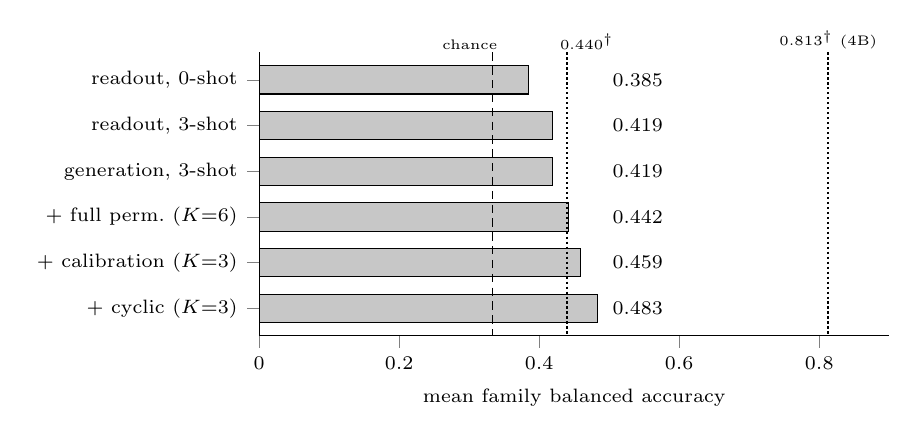
\begin{tikzpicture}
\begin{axis}[
    xbar, scale only axis, width=0.66\columnwidth, height=36mm,
    xmin=0, xmax=0.9, ymin=0.4, ymax=6.6, y dir=reverse,
    bar width=3.6mm,
    ytick={1,2,3,4,5,6},
    yticklabels={{readout, 0-shot},{readout, 3-shot},{generation, 3-shot},{+ full perm.\ ($K{=}6$)},{+ calibration ($K{=}3$)},{+ cyclic ($K{=}3$)}},
    yticklabel style={font=\scriptsize}, xticklabel style={font=\scriptsize},
    xlabel={mean family balanced accuracy}, xlabel style={font=\scriptsize},
    xtick={0,0.2,0.4,0.6,0.8},
    axis lines*=left, tick align=outside, clip=false]
  \addplot[draw=black, fill=black!22] coordinates {(0.38498,1) (0.41937,2) (0.41937,3) (0.44164,4) (0.45948,5) (0.48276,6)};
  % value labels, placed right of every bar and clear of the reference lines
  \node[font=\scriptsize, anchor=west, inner sep=1pt] at (axis cs:0.50,1) {0.385};
  \node[font=\scriptsize, anchor=west, inner sep=1pt] at (axis cs:0.50,2) {0.419};
  \node[font=\scriptsize, anchor=west, inner sep=1pt] at (axis cs:0.50,3) {0.419};
  \node[font=\scriptsize, anchor=west, inner sep=1pt] at (axis cs:0.50,4) {0.442};
  \node[font=\scriptsize, anchor=west, inner sep=1pt] at (axis cs:0.50,5) {0.459};
  \node[font=\scriptsize, anchor=west, inner sep=1pt] at (axis cs:0.50,6) {0.483};
  \draw[densely dashed] (axis cs:0.3333,0.4) -- (axis cs:0.3333,6.6);
  \draw[densely dotted, thick] (axis cs:0.440,0.4) -- (axis cs:0.440,6.6);
  \draw[densely dotted, thick] (axis cs:0.813,0.4) -- (axis cs:0.813,6.6);
  \node[font=\tiny, anchor=south east, inner sep=1pt] at (axis cs:0.345,0.4) {chance};
  \node[font=\tiny, anchor=south west, inner sep=1pt] at (axis cs:0.425,0.4) {0.440$^{\dagger}$};
  \node[font=\tiny, anchor=south, inner sep=1pt] at (axis cs:0.813,0.4) {0.813$^{\dagger}$ (4B)};
\end{axis}
\end{tikzpicture}

\caption{Ablation on authored144 (bars: measured here). Dashed: chance. Dotted ($\dagger$): numbers \emph{published} with the fixture~\cite{openjev} for Qwen3-0.6B and for a 4B model, under a different numeric format, prompt and machine; not measured here. The three debiased bars should not be ranked: cyclic and full permutation are not statistically distinguishable (Sec.~\ref{sec:unresolved}).}
\label{fig:ablation}
\end{figure}

\begin{table}[t]
\caption{Per-family balanced accuracy for the rows of Table~\ref{tab:main} (48 rows per family).}
\label{tab:family}
\centering\footnotesize
\setlength{\tabcolsep}{4pt}
\begin{tabular}{@{}lccc@{}}
\toprule
Method & Candidate sel. & Evidence interp. & Rule appl.\\
\midrule
Readout, 0-shot & 0.430 & 0.356 & 0.369\\
Readout, 3-shot & 0.462 & 0.435 & 0.361\\
Generation, 3-shot & 0.462 & 0.435 & 0.361\\
+ full permutation avg. & 0.484 & 0.329 & 0.512\\
+ calibration (with cyclic) & 0.481 & 0.400 & 0.498\\
+ cyclic permutation avg. & 0.523 & 0.367 & 0.558\\
\bottomrule
\end{tabular}
\end{table}

\textbf{Generation and readout score identically.} Both reach 0.41936868\ldots\ MFBA and 0.465 plain accuracy, with identical per-family values and no unparseable generations (0/144). This is expected: greedy decoding of an answer letter selects the argmax that the readout reads. \emph{The readout therefore does not buy accuracy.} What it buys is closed support (an illegal value cannot be emitted), determinism, and a per-option distribution. We state this plainly because it is the claim a reader is most likely to assume we are making. In this harness the readout run was also 1.19$\times$ faster in wall clock ($225.3/189.6$), a modest difference and, given the timing variance noted below, not one we lean on.

\textbf{The single-ordering readout is close to the published figure.} We measure 0.419 at \code{q4f16}; the published figure is 0.440 in BF16~\cite{openjev}. The gap is in the direction quantisation would predict, but prompts also differ, so we read this only as a sanity check on the harness, not as a finding.

\textbf{Cyclic averaging is worth 6.4 points} ($0.4828-0.4194$), taking the 0.6B model from 0.419 to 0.483. Table~\ref{tab:family} shows the gain is not uniform: rule application rises from 0.361 to 0.558 and candidate selection from 0.462 to 0.523, but evidence interpretation \emph{falls} from 0.435 to 0.367. The per-row predictions of the cyclic run explain why: after the slot prior is averaged away, a \emph{label} prior remains. In evidence interpretation the debiased readout predicts ``supported'' for 45 of 48 rows (gold: 21), and in candidate selection it predicts the option whose identity is ``candidate~B'' (an option id, not the answer letter) for 40 of 48 (gold: 19). Permutation averaging cannot remove a preference attached to an option's content rather than its slot.

\textbf{The model stays order-sensitive.} In the cyclic run, 87 of 144 rows have an argmax identity that differs between rotations. Averaging repairs the \emph{readout}, not the model: of those 87 unstable rows the averaged answer is correct on 39, against 38 of the 57 stable rows (from the per-row prediction file; $39+38=77$ correct, $77/144=0.535$). With calibration applied to each rotation the count is 80 of 144. Under full permutation it is 106 of 144, but that number is not comparable to the other two: six orderings give a row more opportunities to flip than three (Fig.~\ref{fig:instab}). A model that answers partly by position and is corrected afterwards is not the same artefact as one that reads the evidence, and a deployment should not be told otherwise.

\begin{figure}[t]
\centering
% Fig. 6 -- order-unstable rows (argmax identity differs between scored orderings).
% Data: "order_unstable" in
%   bench/results/authored144-...-readout-cyclic-shots3.json      87 / 144  (3 orderings)
%   bench/results/authored144-...-readout-calibrated-shots3.json  80 / 144  (3 orderings)
%   bench/results/authored144-...-readout-full-shots3.json        106 / 144 (6 orderings)
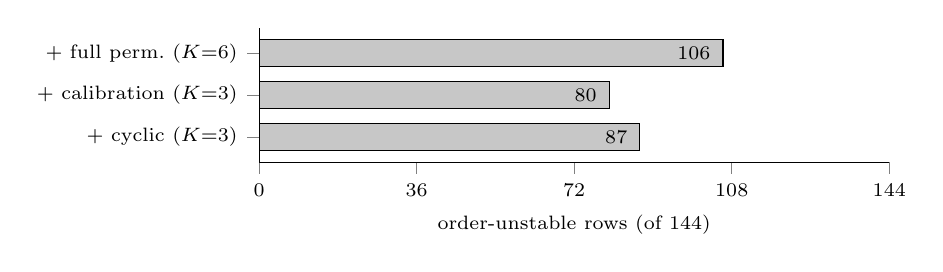
\begin{tikzpicture}
\begin{axis}[
    xbar, scale only axis, width=0.66\columnwidth, height=17mm,
    xmin=0, xmax=144, ymin=0.4, ymax=3.6, y dir=reverse, bar width=3.4mm,
    ytick={1,2,3},
    yticklabels={{+ full perm.\ ($K{=}6$)},{+ calibration ($K{=}3$)},{+ cyclic ($K{=}3$)}},
    yticklabel style={font=\scriptsize}, xticklabel style={font=\scriptsize},
    xtick={0,36,72,108,144},
    xlabel={order-unstable rows (of 144)}, xlabel style={font=\scriptsize},
    nodes near coords, every node near coord/.append style={font=\scriptsize, anchor=east, xshift=-1pt},
    axis lines*=left, tick align=outside]
  \addplot[draw=black, fill=black!22] coordinates {(106,1) (80,2) (87,3)};
\end{axis}
\end{tikzpicture}

\caption{Order-unstable rows. The $K=6$ bar is not directly comparable with the $K=3$ bars (more orderings, more chances to disagree).}
\label{fig:instab}
\end{figure}

\subsection{Cyclic versus full permutation: not distinguishable}\label{sec:unresolved}
Full permutation averaging (six orderings, 0.442) scores \emph{below} cyclic averaging (three orderings, 0.483). The first-order mechanism of Eq.~\eqref{eq:cancel} does not predict a difference: both sets place every option in every slot equally often. In plain accuracy the gap is five rows (77 versus 72 of 144). We therefore re-ran both modes saving per-row predictions and applied the exact McNemar test of Sec.~\ref{sec:setup}. Both methods are right on 69 rows and both wrong on 64; of the \mcnemardiscordant{} discordant rows, \mcnemaronlycyclic{} are correct only under cyclic averaging and \mcnemaronlyfull{} only under full permutation, giving a two-sided $p=\mcnemarp$. \emph{This sample cannot distinguish the two procedures. We report both and do not rank them}; in particular we do not claim that cyclic averaging is better than full permutation averaging, or that fewer orderings are preferable. The test concerns plain per-row correctness rather than MFBA, and this is one model and one fixture. The same caution applies to the calibrated variant (0.459), which lies between them and which we did not test.

Two related remarks. First, the re-runs reproduced the earlier aggregates exactly (0.4828 and 0.4416, identical to every printed digit): nothing is sampled, so on a fixed backend the readout is repeatable. Second, the single-ordering runs were made before per-row predictions were being saved, so we have \emph{not} tested whether the 6.4-point gain of cyclic averaging over the single-ordering readout (77 versus 67 rows correct in plain accuracy) is itself statistically significant.

\subsection{Debiasing does not close the capacity gap}
The best debiased figure we measure for the 0.6B model is 0.483. The published figures on the same fixture and metric are 0.686 for a 2B model and 0.813 for a 4B model~\cite{openjev} (their numbers, different numeric format, prompt and hardware). Option-order priors are a correctable \emph{share} of small-model error; model capacity remains the dominant variable by a wide margin, and a reader choosing a model should weight it accordingly.

\subsection{Shared-prefix reuse is bit-exact in fp32}\label{sec:exact}
\code{bench/shared\_check.mjs} scores five criteria about one state twice---each as a full prompt from scratch, and as suffixes against the once-prefilled head---and reports the maximum absolute difference between the two probability vectors. In fp32 under Node (\code{onnxruntime-node}, CPU) the maximum drift is $0.000\times10^{0}$, i.e.\ the probabilities are identical, for both Qwen3-0.6B and Gemma~3 270M, with all argmaxes agreeing. This contrasts with the BF16 drift the server-side references report (Sec.~\ref{sec:prior}) and suggests that the numeric format, not the method, is responsible for that instability. We did not repeat the check on the WebGPU \code{q4f16} path, where kernels differ, and make no exactness claim there.

\subsection{Cost of a decision}\label{sec:cost}
Following the project's own convention, each statement here is labelled \measured{} (observed on hardware), \derived{} (exact arithmetic from the model configuration, with no timing claim) or \projected{} (an estimate from stated assumptions).

\textbf{Suffix cost is linear (\measured).} Holding a 35-token prefilled state fixed and varying only the suffix length (\code{bench/logit\_cost.mjs}; median over repeats, five by default; CPU backend), the six measured points of Fig.~\ref{fig:suffix} fit by least squares to
\begin{equation}
T_{\text{suf}}(m) \approx 28.4\ \text{ms} + 3.23\ \text{ms}\cdot m ,
\label{eq:fit}
\end{equation}
with residuals under 2\,ms. A typical 45-token criterion is thus \projected{} at $28.4+3.23\cdot45\approx174$~ms on this backend. For scale only: the accuracy harness, which does not reuse the prefix, averaged $189.6/144\approx1.32$~s per three-shot full-prompt pass on the same backend. The two figures come from different prompts and we do not quote their ratio as a speedup.

\begin{figure}[t]
\centering
% Fig. 4 -- suffix length vs latency.
% Data: bench/results/logit-cost-Qwen3-0.6B-q4f16.json  (points_ms, fit)
%   backend: onnxruntime-node, CPU; prefix_tokens = 35; median of 5 repeats per point.
%   fit: 28.4 ms + 3.23 ms/token (least squares over the six points).
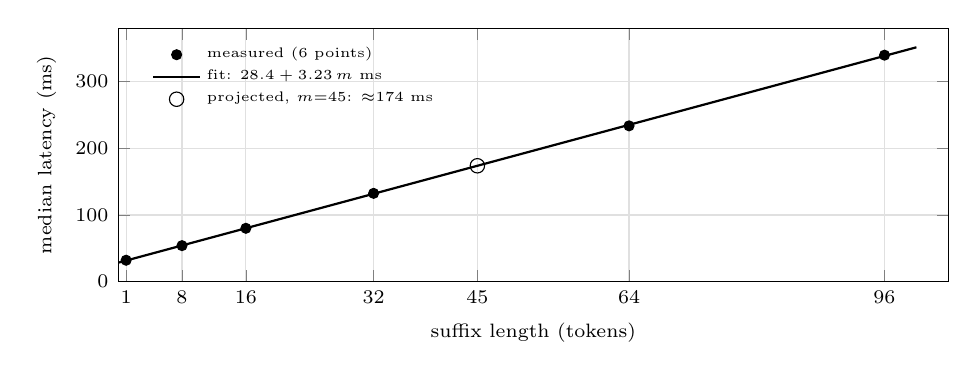
\begin{tikzpicture}
\begin{axis}[
    width=\columnwidth, height=48mm,
    xmin=0, xmax=104, ymin=0, ymax=380,
    xlabel={suffix length (tokens)}, ylabel={median latency (ms)},
    xlabel style={font=\scriptsize}, ylabel style={font=\scriptsize},
    ticklabel style={font=\scriptsize},
    xtick={1,8,16,32,45,64,96},
    legend style={font=\tiny, at={(0.03,0.97)}, anchor=north west, draw=none, fill=none, row sep=-1pt},
    legend cell align=left, grid=major, grid style={black!12}]
  \addplot[only marks, mark=*, mark size=1.8pt, black] coordinates {(1,32.1) (8,54.0) (16,80.0) (32,132.4) (64,233.6) (96,339.6)};
  \addlegendentry{measured (6 points)}
  \addplot[domain=0:100, samples=2, black, thick] {28.4 + 3.23*x};
  \addlegendentry{fit: $28.4 + 3.23\,m$ ms}
  \addplot[only marks, mark=o, mark size=2.6pt, black] coordinates {(45,173.75)};
  \addlegendentry{projected, $m{=}45$: $\approx$174 ms}
\end{axis}
\end{tikzpicture}

\caption{Suffix latency against suffix length, shared prefix held fixed (Qwen3-0.6B \code{q4f16}, \code{onnxruntime-node} CPU). Filled: measured. Open: projection from the fit, not a measurement. Not comparable to WebGPU timings.}
\label{fig:suffix}
\end{figure}

\textbf{Most of the returned logits are unread (\derived).} The stock export has no last-position-only output, so a 45-token suffix returns a tensor of shape $[1,45,151936]$: $45\cdot151936\cdot4 = 27{,}348{,}480$ bytes (27.35~MB, 26.1~MiB) of fp32 per criterion, of which the readout uses $n$ numbers; over one pass of the fixture that is $144\times27.35$~MB $=3.94$~GB. The unembedding accounts for $155{,}582{,}464$ of the model's $596{,}049{,}920$ parameters, so under the usual estimate of two FLOPs per parameter per token it is 26.1\% of per-token compute.

\textbf{What trimming could buy (bounds, not results).} Combining Eq.~\eqref{eq:fit} with the 26.1\% share bounds the effect of an export trimmed to the final position: at least $1.27\times$ if only the unembedding FLOPs of the other 44 positions disappear ($174\to137$~ms), and at most $5.5\times$ if the entire per-token term were logits-related ($174\to32$~ms), which it is not, since attention and MLP work are in that term too. The readback of 0.61~MB per position is not bounded by this arithmetic and depends on the backend. \emph{No trimmed export and no head-pruned export has been built or timed}; these are \derived{} bounds. Likewise \derived: because Qwen3-0.6B ties its input and output embeddings, pruning the head to the answer letters would remove matmul work and logit traffic but essentially nothing from the download.

\subsection{Browser latency: a small advantage, not a large one}\label{sec:browser}
On the demo page (WebGPU, \code{q4f16}, one reference laptop; informal timings recorded in the project README, not a committed benchmark) a ten-criterion rubric about one ticket took about 1.15~s by readout---roughly 90~ms per decision, with the first decision available at about 310~ms. Given a \emph{carefully engineered} prompt (a worked example plus an explicit list of all required keys), the generation lane answered all ten criteria in about 1.5~s, i.e.\ the readout was only about $1.3\times$ faster end to end. With a \emph{merely reasonable} prompt that omitted the key list, the same model returned valid JSON that answered only 4 of the 10 criteria and silently dropped the rest. We report both because the honest latency advantage is small; the practical differences are time to first decision, the impossibility of missing or illegal values, and the per-option probabilities.

% ===========================================================================
\section{The \texttt{typedecide} Library}\label{sec:library}
Stock weights know the format but not a deployer's policy. \code{typedecide} is a Python package for closing that loop; we describe it briefly because it is released with the paper, not because we have results from it. \emph{Bring-your-own-data loaders} read JSONL, JSON, CSV, Parquet and Hugging Face datasets through a column mapping, with strict, diagnostic errors and a validator that flags contradictory labels, class imbalance and inconsistent option sets. \emph{Group splitting}: train/eval splits are made on a grouping key, never on rows, so one state cannot appear on both sides. \emph{Answer-token-only loss}: LoRA~\cite{hu2022lora} training places loss solely on the answer-letter token---the only position the readout reads---truncates long states from the left so the answer slot survives, and randomises option order so that the model cannot learn ``answer A''. \emph{Evaluation} implements Eqs.~\eqref{eq:avg}--\eqref{eq:mfba}, order consistency, ECE and Brier score. \emph{Export} targets ONNX with optional last-position trimming and head pruning (with the tied-embedding untie-before-slice safeguard). Every training run writes a \code{manifest.json} recording base model, resolved configuration, a content hash of the dataset, seed, library versions and the resolved answer-slot ids. The package has more than 250 unit tests, which run without a GPU or model download by using stub tokenizers and models; they test the software, not any scientific claim in this paper.

% ===========================================================================
\section{Limitations and Threats to Validity}\label{sec:limits}
\textbf{What was not done.} No fine-tuned model has been trained or evaluated; the library's training path is exercised by unit tests only. No trimmed export and no pruned export has been built or timed; every statement about them is \derived{} or \projected. A comparison against hosted frontier-model APIs on the same fixture was scripted (\code{bench/api\_baseline.mjs}) but \emph{not run}; we make no claim about it. Constrained decoding was not benchmarked.

\textbf{Sample size and repetition.} All accuracy results are on 144 rows of one fixture with one model. Differences of a few points between debiasing variants are within noise: the one pair we tested, cyclic versus full permutation, is not distinguishable ($p=\mcnemarp$, Sec.~\ref{sec:unresolved}), and the gain of debiasing over the single-ordering readout was not tested because per-row predictions of those runs were not saved. No confidence intervals are reported. The eight-item probe (Table~\ref{tab:probe}) is a signal only, and its outputs are not committed as result files.

\textbf{Fixture.} authored144 is English, synthetic, authored, and model-reviewed rather than human-adjudicated. Nothing here establishes behaviour on real production tickets or other languages. One of our three demonstrations shares option wording with one fixture family.

\textbf{Uncontrolled quantisation and prompts.} Our numbers are \code{q4f16}; published comparison numbers are BF16 with a different prompt. Differences of a few points across that boundary must not be read as model or method differences.

\textbf{Latency.} Timings are single runs on one unspecified, unisolated laptop, and whole-run wall clock is noisy: the committed full-permutation run averages $1442.8/864\approx1.67$~s per scored prompt against $537.3/432\approx1.24$~s for the cyclic run, although the two runs score prompts that differ only in option order; and earlier runs of these two configurations, whose result files have since been overwritten, differed from the committed times by roughly 5\% and 30\%. The Time column of Table~\ref{tab:main} is indicative only. CPU (Node) and WebGPU (browser) figures are not comparable with each other or across machines. Browser timings are informal. The accuracy harness does not use prefix reuse, so Eq.~\eqref{eq:cost} is supported by the suffix-cost measurement, not by an end-to-end timing of debiased readout with reuse.

\textbf{Probabilities are not calibrated confidence.} The readout distribution is conditional on the supplied options. We computed no ECE or reliability analysis on this fixture, and the probabilities should not be thresholded as operational confidence without one.

\textbf{The negative result is stack-specific.} It concerns ONNX Runtime's fused \code{GroupQueryAttention} as reached through transformers.js 4.3.0; no standalone reproduction script is committed, and other runtimes or exports may behave differently.

\textbf{Debiasing is partial.} Permutation averaging removes slot priors only; the label prior documented in Sec.~\ref{sec:results} remains, as does the capacity gap.

% ===========================================================================
\section{Conclusion and Future Work}
Typed logit readout runs in a browser tab on a 0.6B model, at roughly 90~ms per decision on one laptop GPU, with discovered answer slots and bit-exact (fp32) shared-prefix reuse, but without the batched branching that makes the server-side form scale flat. On a public fixture it is exactly as accurate as asking the same model to generate the letter; its advantages are structural. Option-order sensitivity is severe at this scale, invisible to plain accuracy, and partly correctable: cyclic averaging recovers 6.4 points at the price of $K$ short suffixes (full permutation averaging recovers less, but the two are not statistically distinguishable at $n=144$), yet most rows remain order-unstable, a label prior survives, and the result (0.483) remains far from the 0.813 published for a 4B model. The obvious next steps are the ones we have not taken: fine-tune on order-randomised data with answer-token-only loss and measure whether order instability itself falls; build and time trimmed and pruned exports to convert the \derived{} bounds into measurements; evaluate log-space averaging and single-ordering calibration; run the hosted-API comparison; and repeat on larger and non-synthetic fixtures with confidence intervals.

\section*{Reproducibility}
Code, benchmark scripts and the result files cited here are in the project repository, \repourl. The script \code{fetch\_fixtures.sh} in \code{bench/} fetches the fixture from its upstream repository~\cite{openjev}, \code{run\_grid.sh} regenerates every row of Table~\ref{tab:main}, and \code{compare.mjs} runs the McNemar test. Figure sources carry their data inline with the originating result file named in a comment.

\section*{Acknowledgment}
This work builds on a prior open-source implementation~\cite{openjev}, which is not affiliated with and has not endorsed it. Portions of the software, analysis and manuscript text were produced with the assistance of an AI coding assistant (Anthropic's Claude); the author reviewed and takes responsibility for all content.

\bibliographystyle{IEEEtran}
\bibliography{references}

\end{document}
